\part{Algorithms}

\chapter{Introduction}
This report presents the development of a C++ library containing Markov chain sampling algorithms for two major goals: estimation of the density and clustering analysis of a given set of data points.
In a Bayesian nonparametric setting, we focused on the Dirichlet process, one of the most widely used priors due to its flexibility and computational ease, and its extensions.
Hereafter, we will assume that the underlying model for the given data points is a Dirichlet process mixture model, which is an enhancement of the simpler Dirichlet model.
We shall now briefly describe these models and their relevant properties.
(For a more detailed discussion of the nonparametric models, as well as references for all theoretical details included in this section, see \cite{book} chapter 1 and 2.)

\section{Dirichlet process model}
Let $M>0$, and let $G_0$ be a probability measure defined on the state space $S$.
A Dirichlet process with parameters $M$ and $G_0$, noted as $DP(M,G_0)$, is a random probability measure $G$ defined on $S$ which assigns probability $G(B)$ to every set $B$ such that for each finite partition ${B_1,\dots,B_k}$ of $S$, the joint distribution of the  vector $(G(B_1),\dots,G(B_k))$ is the Dirichlet distribution with parameters
\begin{align*}
(MG_0(B_1),\dots,MG_0(B_k)).
\end{align*}
The parameter $M$ is called the precision or total mass parameter, $G_0$ is the centering measure, and the product $MG_0$ is the base measure of the DP. \\
Having observed the independent and identically distributed sample $\{y_1,\dots,y_n\}$ \\*
$\subseteq \RR$, the basic DP model takes the following form:
\begin{equation}
	\begin{aligned}
	y_i | G &\iidsim G, \quad i=1,\dots,n \\
	G &\sim DP(MG_0)
	\end{aligned}
\end{equation}
A key property is that the DP is conjugate with respect to iid sampling, so that the posterior base distribution is a weighted average of the prior base distribution $G_0$ and the empirical distribution of the data, with the weights controlled by $M$:
\begin{align}
	G | y_1,\dots,y_n \sim DP\left(M G_0 + \sum_{i=1}^n \delta_{y_i}\right).
\end{align}
Moreover, the marginal distribution for the data will be the product of the sequence of increasing conditionals:
\begin{align*}
	p(y_1,\dots,y_n)= p(y_1)\prod\limits_{i=2}^{n} p(y_i|y_1,\dots,y_{i-1}),
\end{align*}
with $y_1 \sim G_0$ and the conditional for $i=2,3,\dots$ being the following:
\begin{align*}
	p(y_i|y_1,\dots,y_{i-1})= \frac{1}{M+i-1}\sum_{h=1}^{n-1} \delta_{y_h}(y_i) +\frac{M}{M+i-1} G_0(y_i).
\end{align*}
Another important property is the discrete nature of the random probability measure $G$.
Because of this, we can always write $G$ as a weighted sum of point masses.
A useful consequence of this property is its stick-breaking representation, i.e. $G$ can be written as:
\begin{align*}
	G(\cdot) = \sum_{k=1}^{+\infty} w_k \delta_{m_k} (\cdot),
\end{align*}
with $m_k \iidsim G_0$ for $k\in\mathbb{N}$ and the random weights constructed as $w_k =v_k\prod\limits_{l<k} (1-v_l)$ where $v_k \iidsim Be(1,M)$. \\
In many applications in which we are interested in a continuous density estimation, this discreteness can represent a limitation.
Oftentimes a Dirichlet process mixture (DPM) model is used, where the DP random measure is the mixing measure for the parameters of a parametric continuous kernel function.

\section{Dirichlet process mixture model}
Let $\Theta$ be a finite-dimensional parameter space and $G_0$ a probability measure on $\Theta$.
The Dirichlet process mixture (DPM) model convolves the densities $f(\cdot|\boldsymbol\theta)$ from a parametric family $\Fc = \{f(\cdot|\boldsymbol\theta), \boldsymbol\theta \in \Theta \}$ using the DP as mixture weights.
The obtained model has the following form:
\begin{equation}
	\begin{aligned}\label{dpm-1}
	y_i | G &\iidsim f_G(\cdot) = \int_\Theta f(\cdot|\boldsymbol\theta) \, G(\de\boldsymbol\theta), \quad i=1,\dots,n \\
	G &\sim DP(M G_0)
	\end{aligned}
\end{equation}
An equivalent hierarchical model is:
\begin{equation}
	\begin{aligned}\label{dpm-2}
	y_i | \boldsymbol\theta_i &\indsim f(\cdot|\boldsymbol\theta_i), \quad i=1,\dots,n \\
	\boldsymbol\theta_i | G &\iidsim G, \quad i=1,\dots,n \\ 
	G &\sim DP(M G_0)
	\end{aligned}
\end{equation}
where the \emph{latent variables} $\boldsymbol\theta_i$ are introduced, one per unit.
Since $G$ is discrete, we know that two independent draws $\boldsymbol\theta_i$ and $\boldsymbol\theta_j$ from $G$ can be equal with positive probability.
In this way the DPM model induces a probability model on clusters of $\boldsymbol\theta_i$.
An object of interest that derives from this model is the partitioning induced by the clustering. \\%, as well as the density estimation. \\
Considering $n$ data points, each $\boldsymbol\theta_i$ will have one of the $k$ unique values $\boldsymbol\phi_{j}$.
An estimation of the number of the unique values is $M\log(n) \ll n$.
Defining  $\boldsymbol c= (c_1,\dots,c_n)$ the \emph{allocation} parameters to the clusters such that $c_i = j$ if $\boldsymbol\theta_i = \boldsymbol\phi_j$, model (\ref{dpm-2}) can be thought of as the limit as $K \to +\infty$  of a finite mixture model with $K$ components (recall instead that $k$ is the number of unique values):
\begin{equation}
	\begin{aligned}\label{dpm-disc}
		y_{i}|\boldsymbol{\phi}_1,\dots,\boldsymbol{\phi}_k,c_{i} &\indsim f(\cdot|\boldsymbol\phi_{c_{i}}), \quad i=1,\dots,n \\
		c_{i}|\mathit{\mathbf{p}}&\iidsim \sum_{j=1}^K\mathit{p_j} \delta_j(\cdot), \quad i=1,\dots,n \\
		\boldsymbol\phi_{c} & \iidsim G_{0}, \quad c=1,\dots,k \\
		\mathbf{p} &\sim \operatorname{Dir}(M/K,\dots,M/K)
	\end{aligned}
\end{equation}
where $\mathbf{p}=(p_1,\dots,p_K)$ represents the mixing proportions for the clusters and each $\boldsymbol\theta_i$ is characterized by the latent cluster $c_i$ and the corresponding parameters $\boldsymbol\phi_{c_i}$.

\subsection{Normal Normal-InverseGamma model} \label{nnig}
A very common choice for the DPM model (\ref{dpm-1}) is the Normal Normal-InverseGamma (Normal-NIG) model, opting for a Normal kernel and the conjugate Normal-InverseGamma as base measure $G_0$. That is, letting $\boldsymbol\theta=(\mu,\sigma)$, we have:
\begin{equation}
	\begin{aligned}
		f(y|\boldsymbol\theta)&=N(y| \mu ,\sigma^2),  \\
		G_0(\boldsymbol\theta|\mu_0,\lambda_0, \alpha_0, 	\beta_0)
		&=N\left(\mu | \mu_0 ,\frac{\sigma^2} {\lambda_0}\right) \times \text{Inv-Gamma}(\sigma^2|\alpha_0, \beta_0 ).
	\end{aligned}
\end{equation}
Note that in this model we have a full prior for $\sigma^2$ and instead a prior for $\mu$ that is conditioned on the value of $\sigma^2$.
Thanks to conjugacy, the predictive distribution for a new observation $\widetilde{y}$ can be computed analytically, finding a Student's $t$ (see \cite{integral} section 3.5):
\begin{align*}
	p(\widetilde{y}|\mu_0,\lambda_0, \alpha_0, \beta_0) =
	\int_\Theta f(\widetilde{y}|\boldsymbol\theta) \, G_0(\de\boldsymbol\theta) =
	\text{t}_{\widetilde \nu}\left(\widetilde{y}|\widetilde{\mu},\widetilde{\sigma}\right)
\end{align*}
where the following parameters are set:
$$
	\widetilde{\nu}=2 \alpha_0, \quad
	\widetilde{\mu}=\mu_0, \quad
	\widetilde{\sigma}^2= \frac{\beta_0(\lambda_0+1)}{\alpha_0 \lambda_0}
$$
Moreover, the marginal distribution for a given observation has the same expression. \\
The posterior distribution is again a Normal-InverseGamma (see \cite{integral} section 3.3):
\begin{align*}
	p(\boldsymbol\theta|y_1,\dots,y_n,\mu_0,\lambda_0, \alpha_0, \beta_0)=N\left(\mu | \mu_n ,\frac{\sigma^2} {\lambda_0 + n}\right) \times \text{Inv-Gamma}(\sigma^2|\alpha_n, \beta_n )
\end{align*}
with:
$$
\mu_n=\frac{\lambda_0 \mu_0 \bar{y} + n}{\lambda_0 + n}, \quad \alpha_n= \alpha_0 + \frac{n}{2}, \quad \beta_n= \beta_0 + \frac{1}{2}\sum_{i=1}^{n} (y_i-\bar{y})^2 + \frac{\lambda_0 n(\bar{y}-\mu_0)^2}{2(\lambda_0 + n)}.
$$

\chapter{Algorithms} \label{algo}
For the task of density estimation, we investigated several Markov chain methods to sample from the posterior distribution of a DPM model. \\
Starting from the hierarchical model (\ref{dpm-1}), a first direct approach is simply drawing values for each $\boldsymbol\theta_i$ from its conditional distribution, given the data and the other $\boldsymbol\theta_j$.
However, as previously discussed, we have high probability for ties among them which can lead to slow convergence, since the $\boldsymbol\theta_i$ are not updated for more than one observation simultaneously. \\
For this reason, special attention was paid to the three methods we present in this chapter.
They are Gibbs samplers with a similar base structure, sharing the two steps for the sampling of the allocations $\mathbf{c}$ and of the unique values $\boldsymbol\phi_c$.
The set of allocations and unique values at a given iteration constitutes the \emph{state} of that iteration.
As the state is being updated at each iteration, a \emph{chain} is formed and the mean of the state values eventually reaches convergence, as well as the estimate for the data distribution, as we will see in section \ref{dens-estim}.
Moreover, all methods can be extended with additional steps for hierarchical extensions.
For example, we can place priors to hyperparameters of the centering measure $G_0$ or to the total mass $M$.

\section{Neal's Algorithm 2} \label{neal2}
In order to speed up convergence in case of ties, Neal first proposed (see \cite{neal} section 3 as well as \cite{book} chapter 2) a more efficient Gibbs sampling method based on the discrete model (\ref{dpm-disc}), but where the mixing proportions $\textbf{p}$ have been integrated out.
We will refer to this method as Neal's Algorithm 2, or \verb|Neal2| for short.
Before getting to the algorithm, let us start from the discrete model (\ref{dpm-disc}).
Assuming that the current state of Markov chain is composed of $(c_1,\dots,c_n)$  and the unique values $\boldsymbol\phi_c$ for all $c=1,\dots,k$, the Gibbs sampler should first draw a new value $c$ for each $c_i$ according to the following probabilities:
\begin{align}
	\hspace{-25pt}
	\vspace{-12pt}
	\text{If $c=c_j$ for some $j$: }
	\PP(c_{i}=c | \boldsymbol c_{-i}, y_{i},\boldsymbol{\phi}_1,\dots,\boldsymbol{\phi}_k) \propto \frac{n_{-i,c} + M/{K}}{n-1+M} f(y_{i}|\boldsymbol\phi_{c}) 
\end{align}
where $\boldsymbol c_{-i}$ is $\boldsymbol c$ minus the $i$-th component, and $n_{-i,c}$ is the number of $c_j$ equal to $c$ excluding $c_i$.
The transition to the infinite case, that is, to the reference DPM model (\ref{dpm-2}), is handled by taking the limit as $K$ goes to infinity in the conditional distribution of $c_i$, which becomes as follows:
\begin{equation}
	\begin{aligned} \label{probasneal2}
	\hspace{-25pt}
	\vspace{-12pt}
	\text{If $c=c_j$ for some $j$: }
	\PP(c_{i}=c | \boldsymbol c_{-i}, y_{i}, \boldsymbol{\phi}_1,\dots,\boldsymbol{\phi}_k) &\propto \frac{n_{-i,c} }{n-1+M} f(y_{i}|\boldsymbol\phi_{c}) \\
	\PP(c_{i}\neq c_{j} \text{ for all } j | \boldsymbol c_{-i}, y_{i}, \boldsymbol{\phi}_1,\dots,\boldsymbol{\phi}_k) &\propto \frac{M }{n-1+M} \int_{\Theta} f(y_{i}|\boldsymbol\theta) \, G_0(\de\boldsymbol\theta)
	\end{aligned}
\end{equation}
and considering only the $\boldsymbol\phi_c$ associated with some observation, keeping the sampling finite and thus computationally feasible.
The former expression is proportional to the cardinality of that cluster (excluding the $i$-th observation), while the latter is instead proportional to the total mass $M$ and represents the probability of creating a new cluster.
Moreover, the integral $m(y_i) = \int_{\Theta} f(y_{i}|\boldsymbol\theta) \, G_0(\de\boldsymbol\theta)$ represents the \emph{marginal distribution} of the data points evaluated in $y_i$. \\
Let us now introduce the actual \verb|Neal2| algorithm, which works iteratively in two steps, in which we sample $(\boldsymbol{c}_1,\dots,\boldsymbol{c}_n)$ and $(\boldsymbol{\phi}_1,\dots,\boldsymbol{\phi}_k)$, respectively.
First, for each observation $i$, $c_i$ is updated according to the conditional probabilities (\ref{probasneal2}).
It can be set either to one of the other components currently associated with some observation, or to a new mixture component.
If the new value of $c_i$ is different from all the other $c_j$, a value for $\boldsymbol\phi_{c_i}$ is created by drawing it from the posterior distribution $H_i$, given the prior $G_0$ and the single observation $y_i$; this means that in this case, a new cluster has been created. \\
Then, for all clusters, the sampling of their unique value $\boldsymbol\phi_c$ is conducted by considering their posterior distribution given the prior $G_0$ and all observations belonging to that cluster.
The probability of setting $c_i$ to a new component involves the computation of the marginal, which is difficult to compute in the non-conjugate case, as well as the sampling from the posterior $H_i$.
For this reason, the algorithm is only used under conjugacy and hence it is possible to exactly compute the integral.

\section{Neal's Algorithm 8} \label{neal8}
To handle non-conjugate priors, Neal proposed (see \cite{neal} section 6 and \cite{book} chapter 2) a second Markov chain sampling procedure, the \verb|Neal8| algorithm, where the state is extended by the addition of $m$ auxiliary parameters.
This technique allows to update the $c_i$ while avoiding the integration with respect to $G_0$ for the computation of the marginal. \\
In this case the sampling probabilities for the $c_i$ given all other $c_j$ are:
\begin{equation}
	\begin{aligned}
		\hspace{-25pt}
		\vspace{-12pt}
		\text{If $c=c_j$ for some $j$: } \PP(c_i=c | \boldsymbol c_{-i}) &= \frac{n_{-i,c}}{n-1+M}   \\
		\PP(c_{i}\neq c_{j} \text{ for all } j) &=\frac{M }{n-1+M}
	\end{aligned}	
\end{equation}
where the latter probability of creating a new cluster is evenly split among the $m$ auxiliary components, which will also be referred to as the \emph{auxiliary blocks}.
Maintaining the same structure as the \verb|Neal2| algorithm, \verb|Neal8| is composed of two steps, where the components of the Markov chain state $(\boldsymbol{c}_1,\dots,\boldsymbol{c}_n)$ and $(\boldsymbol{\phi}_1,\dots,\boldsymbol{\phi}_k)$ are repeatedly sampled.
\begin{figure}[h]
    \centering
    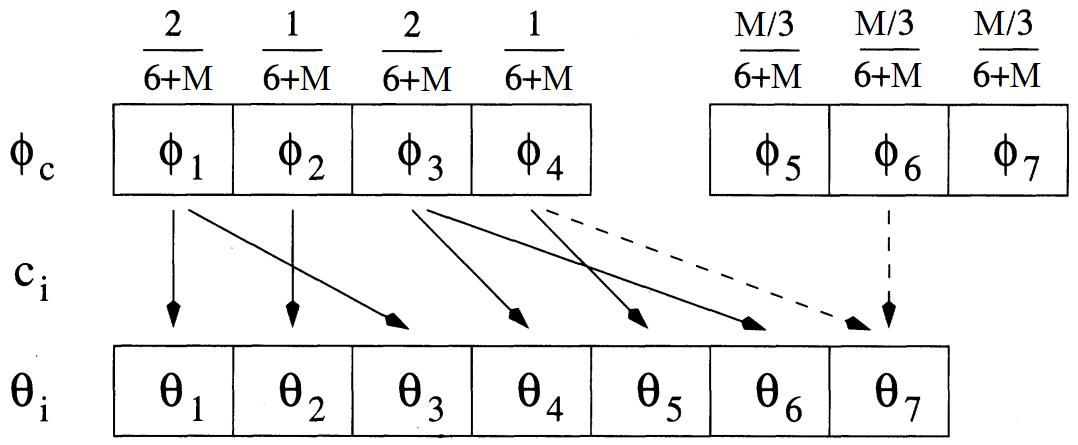
\includegraphics[width=0.9\textwidth]{etc/neal8.png}
    \captionsetup{labelformat=empty}
    \caption{Graphical representation of the variables: the allocations are visualized as arrows linking each $\boldsymbol\theta_i$ with either one of the four old clusters or one of the new components (image taken from \cite{neal})}
    \label{fig:neal8}
\end{figure}

The first step scans all the observations and evaluates each $c_i$.
If it is equal to some other $c_j$, i.e. if the current cluster of observation $i$ is not a singleton, then all auxiliary variables are iid drawn from $G_0$.
If instead the cluster corresponding to $c_i$ is a singleton, then it is linked to one of the auxiliary blocks (i.e. the first one, without loss of generality) while keeping its old unique value $\boldsymbol\phi_{c_i}$ (as shown in the above figure), whereas the other blocks are drawn normally from $G_0$ as before.
Then, $c_i$ is updated according to the following conditional probabilities:
\begin{equation}
	\begin{aligned} \label{neal8prob}
		\PP(c_{i}=c | \boldsymbol c_{-i}, y_{i}, \boldsymbol\phi_{1},\dots,\boldsymbol\phi_{h}) \propto
		\begin{cases}
			\dfrac{n_{-i,c}}{n-1+M}f(y_{i}|\boldsymbol\phi_{c}), & \mbox{for } 1 \leq c \leq k^{-} \\
			\\
			\dfrac{M/m}{n-1+M}f(y_{i}|\boldsymbol\phi_{c}), & \mbox{for } k^{-}+1 < c \leq h,
		\end{cases}
	\end{aligned}
\end{equation}
indicating with $k^{-}$ the number of distinct $c_j$ excluding the current $c_i$ and setting $h=k^{-}+m$.
Again, the probabilities of being placed in an already existing cluster or in a newly created cluster are proportional to the cluster's cardinality (sans observation $i$) and to the total mass, respectively. \\
Once all the $\boldsymbol\phi_c$ that are no longer associated with any observation are discarded, the algorithm proceeds, for each cluster, with the sampling of $\boldsymbol\phi_c$ from the posterior computed with the observations of the specific cluster, similarly to the \verb|Neal2| algorithm.

\section{Blocked Gibbs}
Another Gibbs sampling method that is applicable in the considered DPM model is the one proposed by Ishwaran and James (see \cite{james} section 5), where the prior $P$ is assumed to be a finite dimensional stick-breaking measure, allowing the update of whole blocks of parameters.
A key point of the method is that it does not marginalize over the prior; instead, by grouping more variables together, it samples from their joint distribution conditioned on all other variables.
This sampler needs to draw from the following conditionals:
\begin{align}
	\boldsymbol\phi_1,\dots,\boldsymbol\phi_k &\sim \Lc(\cdot | c_1,\dots,c_n, \boldsymbol{y}) \nonumber \\
	c_1,\dots,c_n &\sim \Lc (\cdot | \boldsymbol\phi_1,\dots,\boldsymbol\phi_k,\boldsymbol{p}, \boldsymbol{y}) \nonumber \\
	\boldsymbol{p} &\sim \Lc (\cdot | c_1,\dots,c_n) \nonumber
\end{align}
The drawing of the unique values can also be handled in the non-conjugate case by applying standard Markov chain Monte Carlo methods. \\
This algorithm is not explored in detail as it has not implemented yet in our library.
For a full explanation, see \cite{james}.
